\subsection{Model structure}

% Teksten vår presenterer et vitkig punkt med model structure
% Her er det spessielt vekt på lokale vs globale metoder
% I tillegg til univariate vs multivariate

% Vi reffererer bare til teori bak dette, og denne er litt uklar
% Pressisere at vi ikke har noe perfekt data på om data henger sammen eller ikke
% Det er mulig at noe av dataen vi har har en sterk korrelasjon, mens andre deler av dataen ikke hører sammen i det hele tatt.
% Det kan være vanskelig å si.
% Vi har teori bak hvorfor de ulike methodene kan være gunstige og ugunstige
% Det blir viktig å få frem begge disse aspektene når det skal diskuteres

% For at dette skal skilde seg ut fra "related work" er det viktigere at vi ser dette i forhold til vår foreslåtte oppgave / framework
% Hvorfor vil disse ulike data modellene utgjøre en forskjell når det kommer til vår modell
% Hvorfor er vår data godt egnet, og mulig ikke godt egnet til dette'
From what we learned from \Cref{section:RelatedWork:Model-structure}
there are many possible ways of constructuring a model.

A local univariate approach would be similar to how an ARIMA model would work.
It would benefit from being simple, but to forecast $n$ product categories,
one would need $n$ models.
The benefit of having $n$ models is that consumer product categories are a dynamic set, constantly changing.
When a new category of products is created, a forecasting model is created with it. Its forecasting ability
would be limited but would gradually improve as more data accumulated.

\begin{figure}[h!]
  \centering
  \caption{TODO}
  \label{fig:model-structure-examples}
  \begin{subfigure}[b]{0.4\textwidth}
    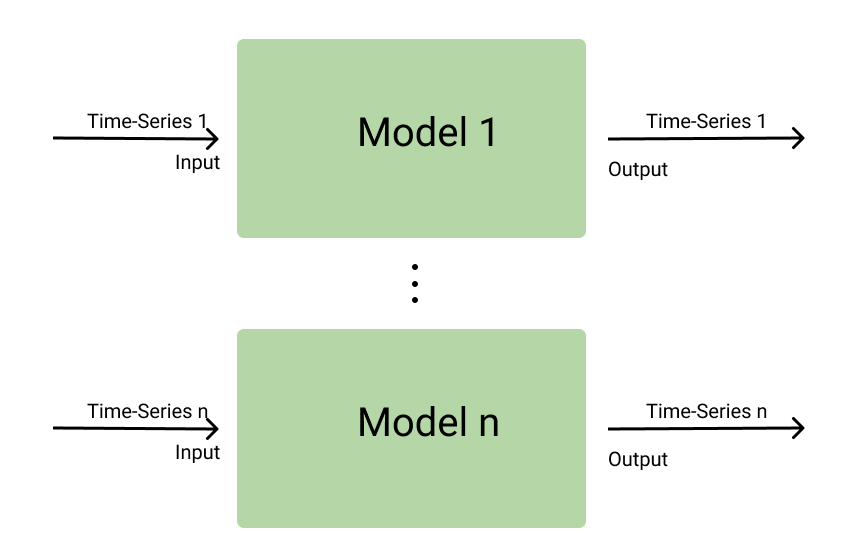
\includegraphics[width=\textwidth]{./figs/illustrations/illustration_local_univariate.png}
    \hfill
    \caption{Local univariate}
    \label{fig:model-example-local-univariate}
  \end{subfigure}
  \begin{subfigure}[b]{0.4\textwidth}
    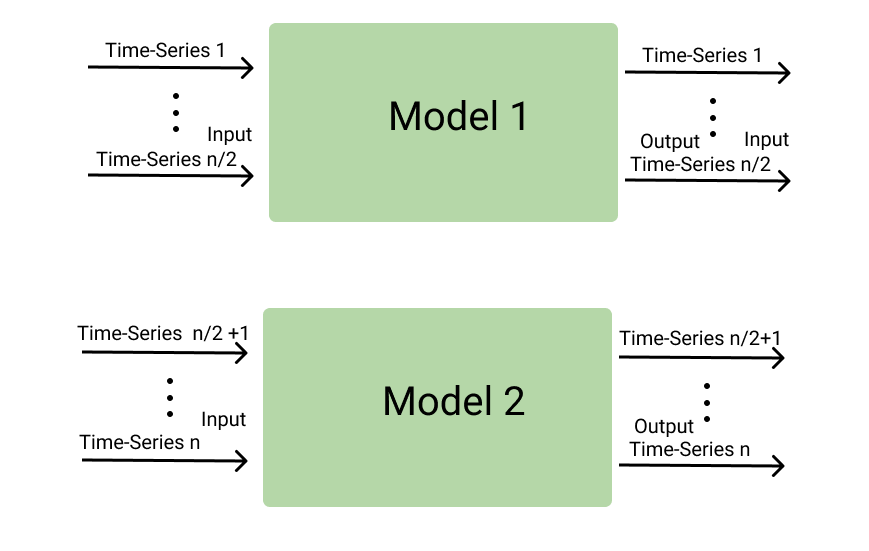
\includegraphics[width=\textwidth]{./figs/illustrations/illustration_local_multivariate.png}
    \hfill
    \caption{Local multivariate}
    \label{fig:model-example-local-multivariate}
  \end{subfigure}
  \begin{subfigure}[b]{0.7\textwidth}
    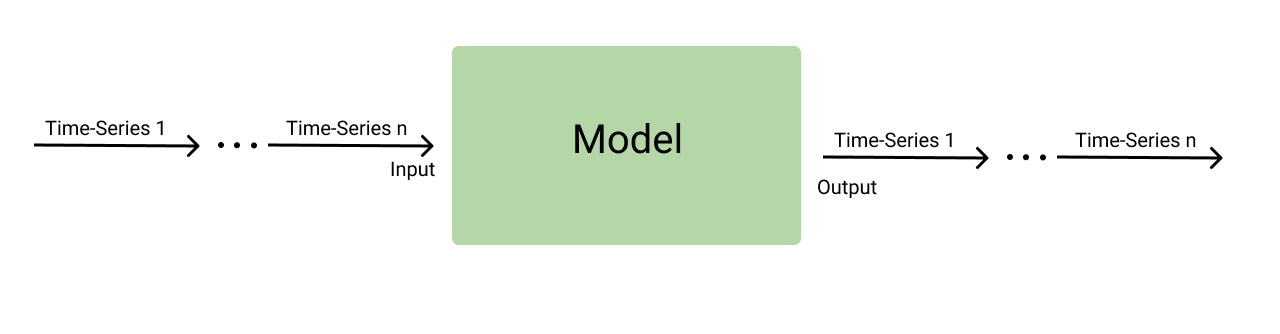
\includegraphics[width=\textwidth]{./figs/illustrations/illustration_global_univariate.png}
    \hfill
    \caption{Global univariate}
    \label{fig:model-example-global-univariate}
  \end{subfigure}
\end{figure}

The greatest drawback of a local univariate approach would be the assumption that all product categories
are independent. We can expect some groups to correlate with each other. These interdependent relationships
could significantly improve forecasting ability.

A multivariate approach will capture these relationships.
However, one needs a thorough understanding of the underlying data to build meaningful models.
A thorough covariance analysis to identify correlating groups of product categories would be best.
%However, this might be outside of scope(?).
The work proposed by \cite{Sen2019} has the advantage of capturing interdependent time-series features and dealing with
some of the drawbacks of a multivariate model. However, their model is intended for as many time series as up to millions.
This is to vastly over-engineer our problem.
%They solution is also based on a temoral convolution network.

A multivariate model does have some drawbacks in an ever-changing product category domain.
First, it's the issue that not all categories have the same life of existence, and thus a variable
amount of history data would amount to many null values.
Second, each time a category is added or changed, a covariance analysis has to be done to identify
which covariance group the category belongs to. Then that model has to be retrained.
Depending on the number of changes to the category tree, this might hinder.

The univariate global approach has the benefit of overcoming many of the hindrances of a multivariate model.
It does not care which product category you feed it, so it is very scalable. The argument given by\cite{Bandara2017},
that a single global model might be detrimental to overall accuracy, could be overcome by clustering product categories together.
This is true even if \cite{Rabanser2020}
shows that global models will improve accuracy, even if the global model assumption is not satisfied.

Another question is how such a cluster of product categories is to be made.
\cite{Bandara2017} suggests a K-means clustering technique
which looks at several time series characteristics, such as
strength of a trend, the strength of spikiness, strength of curvature,
and sales quantile.

The global method will not capture interdependent relationships directly
but might do so indirectly. It also has the potential to build a lot more complicated model,
as the amount of training data will drastically increase, which again will make the model less prone to
overfitting.

% Should this be under multi vs univariate section?
% Currently it does not have any references
One last approach is to build a multivariate model which only forecasts a single product category at the time.
The input to such a model might be a decomposition of the target time series.
For example, decomposing a time series into a component that shows how the series's trend behaves over time,
one component for the cycles, and one for noise.
Another option is to rely on external data sources which correlate with the target series.
For example, it is to be expected that if a product category group suddenly spikes in interest at Prisguiden.no,
then a similar spike would happen at Google.
Or bad weather might affect interest rates at Prisguiden because people are inside on the computer more.
Such a method can also have the additional benefit of being a global model.
This is precisely what \cite{Laptev} did, and they achieved a promising result.

To conclude, it is unclear what the best model would be for our case.


%This apprach would also be hard to scale. If one 

% Global models
% + scalable
% + Can use complicated models because of a lot of training data
% + Has seen some promesing results resently
% - Might miss interdependent relationships
% - A single global model might be too general
% Could split into sub groups

% Multivariate models
% + Can see interdependent relationships between time series
% - Difficult to scale, as adding one category means changing the models 
% shape
% Will maximize the effectiveness of CNN?
